\chapter{估算软件规模} % Introduction chapter suppressed from the table of contents


\hypertarget{ux4e3aux4ec0ux4e48ux8981ux4f30ux89c4ux6a21}{%
\subsection{为什么要估规模}\label{ux4e3aux4ec0ux4e48ux8981ux4f30ux89c4ux6a21}}

规模可以帮我们:

\begin{enumerate}
\tightlist
\item
  依据历史数据策划,例如估算工作量、工期
\item
  归一(Normalize)不同项目,作比较
\item
  知道现在水平
\end{enumerate}

依据历史数据策划 先把项目分成组件,参考以往类似的组件所花工作量,估算整个项目的总工作量。规模大小可简单看成是组件的数量。 (如果是新开发,以前从未做过同类开发,就只能靠个人经验直接估算工作量(或工期), 但是如果以前做过类似的工作,就可以参考以前的历史数据估算。) 
规模可以帮我们把不同项目归一。例如,验收测试缺陷数无法比较,但缺陷率 (
=缺陷数 / 规模) 便可以比较; 生产率(= 规模 / 所花总工时) 便可比。

有了归一后可比较的系数,个人/团队便更清楚当前的水平(质量/生产率),是否在上升或下降。

\hypertarget{ux4e3aux4ec0ux4e48ux4e0dux5e94ux7528ux4ee3ux7801ux884cux6570loc}{%
\subsection{为什么不应用代码行数(LOC)}\label{ux4e3aux4ec0ux4e48ux4e0dux5e94ux7528ux4ee3ux7801ux884cux6570loc}}

在1996年前, IBM 一直使用代码行数估算规模。
之前一直都使用近似机器语言的Assembly Lang.,
但为了提升效率,引入了高层语言 PL/S,发现 不能再用代码行数来估算规模
因PL/S 只需要更少代码行数 也能完成同样功能:

%Screenshotfrom20221220202712.png

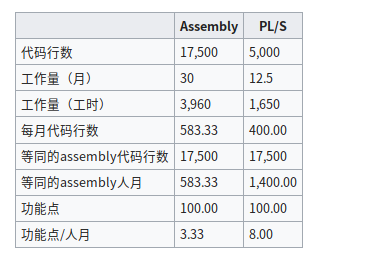
\includegraphics[width=10cm]{Screenshotfrom20221220202712.png}

上表是IBM(1968 - 1975)对两种编译器的统计:\\
每个月 PL/S产出代码行数(400) 反比 Assembly(583) 少

但是如果用功能点数便能真正反映生产率的提升: PL/S : 8.00 对比 Assembly
:3.33

\hypertarget{ux53eaux9002ux7528ux4e8eux7f16ux7801}{%
\subsubsection{只适用于编码}\label{ux53eaux9002ux7528ux4e8eux7f16ux7801}}

看下表,代码行数只能反应编程的工作量,但编码仅占项目总工作量的一部分
如果把项目按工作量分成以下五个部分 代码行数只能用于第二部分编码 (25\%)
其他4部分(30\% + 20\% + 15\% + 10\%)都不合适。

%Screenshotfrom20221220202832.png

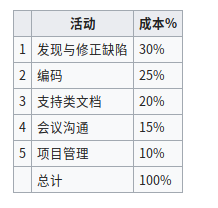
\includegraphics[width=10cm]{Screenshotfrom20221220202832.png}

\hypertarget{ux4e0eux529fux80fdux70b9ux6bd4ux8f83}{%
\subsubsection{与功能点比较}\label{ux4e0eux529fux80fdux70b9ux6bd4ux8f83}}

能估算好项目规模应可帮助我们更好估算工作量,规模应具备以下条件:

\begin{enumerate}
\tightlist
\item
  要和工作量有密切相关 - 应该与工作量强相关
\item
  要容易数得出来
\item
  容易在项目早期可以估算到
\end{enumerate}

功能点比较符合以上条件;只要功能需求明确,就可以估算出对应的功能点数。

只要需求明确便可以准确客观的估算功能点数。
因功能点估算已经是国际标准,基于功能点的度量数据可以与其他国家的标杆对比。

\hypertarget{ux600eux6837ux4f30sifp}{%
\subsection{怎样估SiFP}\label{ux600eux6837ux4f30sifp}}

有了功能性需求,并识别出系统范围,就可以开始估算功能点。:

\begin{enumerate}
\tightlist
\item
  数据功能(简称`实体')的数量 * 7 (实体是系统要管理的数据,)
\item
  业务功能(简称`行为')的数量 * 4.6 (行为可以简单看成是增删改查等功能)
\end{enumerate}

\begin{description}
\tightlist
\item[]
简化功能点数 = 上面 1 和 2 的总数
\end{description}

例如,附件例子一:潜水学校新开发项目:

\begin{itemize}
\tightlist
\item
  识别出3个实体和24个行为,得出简化功能点数131.4 = 3 * 7 + 24 * 4.6
\end{itemize}

潜水学校二次开发项目:
有些功能删除,有些功能变更,就需要分开计算动态功能点和静态功能点:

\begin{itemize}
\tightlist
\item
  静态功能点可以看成是整个系统的功能点数,所以变更的功能点数不会引起影响,但删除的话就需要减去。
\item
  动态功能点主要是用于估算本期开发项目的工作量,因为无论变更功能或者删除功能,都会导致有开发工作量,所以不能是零或负数。国际功能点的规定很简单,都加起来。
\end{itemize}

所以这次二次开发的动态功能点是:

\begin{description}
\item[]
\begin{description}
\tightlist
\item[]
2 * 7 + 11 * 4.6 (增加 两个实体和十一个行为)
\end{description}

+ 1 * 7 + 3 * 4.6 (变更 一个实体和三个行为)

+ 0 * 7 + 2 * 4.6 (删除 两个行为)

= 64.6 + 20.8 + 9.2
\end{description}

再加上 4.6 (因为有数据转换,所以需要加一个CFP,等于4.6)\\
最终动态功能点是99.2 (= 64.6 + 20.8 + 9.2 + 4.6)

静态功能点: 新开发 , 加上新增, 减去删除的功能点

\begin{description}
\item[]
\begin{description}
\tightlist
\item[]
= 131.4 + 64.6 - 9.2

= 186.6
\end{description}
\end{description}

\hypertarget{ux4eceux6545ux4e8bux70b9ux8f6cux7b80ux5316ux529fux80fdux70b9}{%
\subsection{从故事点转简化功能点}\label{ux4eceux6545ux4e8bux70b9ux8f6cux7b80ux5316ux529fux80fdux70b9}}

因故事点只是每个团队自己定义,无法用来作为组织级标准衡量规模,所以很多公司(尤其是银行)转用功能点来衡量软件开发规模。它不仅可用于公司内,也适用于行业标杆,功能点也适用于公司内或公司间结算,例如软件维护期里开发工作量变化很大,也难以事前预估,所以有些银行会按最终开发出来的功能点数结算使用部门付开发部的费用,减少争议。

虽然功能点分析源自70年代,但由于计算较复杂,一直未普及,有些人觉得IFPUG
FPA太复杂。针对这问题,国际功能点协会简化本来的功能点算法,推出简化功能点(SiFP),减少了估算的工作量与学习难度(例如,培训可以从以往的2天半降到半天)。因简化功能点不考虑实体/行为的复杂度,它与本来功能点的估算有\(\pm\)
15 \textasciitilde{} 20\% 偏差(详见附件例子)。
因敏捷团队是按每轮迭代估算(而不是一次性估整个项目),偏差就可以接受
(例如,2周一个迭代,偏差大概1.5天),所以SiFP
能适用于敏捷多次迭代估算。所以越来越多团队开始从故事点转简化功能点,但由于不熟识功能点估算是从用户角度估算,而非从开发工程师的视角看,团队初次估算SiFP通常有误。下面是某成都团队从故事点转简化功能点的案例:

\framebox{%
\begin{minipage}[t]{0.97\columnwidth}\raggedright
客户:我们以前一直使用故事点,为了更好做量化管理,我们新的项目开始使用简化功能点
- SiFP\\
我:好的,看一下你的估算表 。 。 。 。
为什么这两个功能要分成两个行为?\\
客户:这两个功能都挺复杂,估计需要很多开发工作量;我们以前用故事点估算时,也会分成两个故事点。\\
我:请注意,在功能点估算, 是否是一个行为,取决于它算不算是一个基本过程
如果俩行为互相依赖,不能单独作为基本过程,就不应该分开为2个功能点。很多团队刚开始用功能点,与你们一样,没有弄清楚基本过程的概念,还是从工程师的角度,估计开发时间的工作量来判断是一个功能还是两个功能?在故事点用这种方式估算习惯,但因为功能点是要同一个功能上需求,不能有功能点数的差异,所以不能用估计开发难易程度来判断。\\
客户:可否举个实例?\\
我:以网约车为例,是否可以分成以下9个''行为``?

%\href{文件:sifp_p50图.jpg}{600px}

\includegraphics[width=10cm]{sifpp50图.jpg}

\begin{enumerate}
\tightlist
\item
  预约申请
\item
  接收预约
\item
  检查是否有可用的车/司机
\item
  寻找其他可选
\item
  提供预约信息
\item
  处理预约
\item
  分派司机
\item
  接乘客
\item
  完成预约请求
\end{enumerate}

客户:是的,每个行为都要花一定开发工作量。\\
我:其实按SiFP只有4个行为,因头5个,和最后2个都要合并才可以成行为(详见附件)。
如果要能独立成行为,必须符合基本过程条件。
基本过程不是随便定的,它有规则,比如从网约车案例我们可以看到,``预约申请''本身不能算一个基本过程,虽然预约申请可能要很复杂的开发工作,但是因为它不能独立存在,必须依赖其它的行为才算完整。\\
例如,某公司财务系统有打印支票功能(用来付供应商),你觉得打印支票本身是否算基本过程?\\
客户:听完你网约车例子,应该不算;因打印支票只是付款流程的一个可选部分。\\
我:正确、算实体也应使用同样概念。例如,某人事管理系统,除了管理职工信息外,还有员工家属信息,因家属信息必须关连到员工信息,不能独立存在,所以家属信息本身不算是一个实体。你是否觉得你这表里的某些实体应合并?\\
客户:听完你的解释,同意我们这次计算有些实体应合并。\\
我:你们的功能点估算表没有明确区分新的迭代怎么处理变更与删除。
也没有明确动态功能点与静态功能点。\\
客户:我们表中有计算每次迭代的总功能点数。\\
我:你们可能有算每迭代的功能点,但难以看清后面迭代对应之前的变化。动态功能点是用来估算本本迭代的工作量,而静态功能点就是迭代后产品的功能点数。而且应该用表格形式把变更和删除累加在原本上一轮的功能上面,才可以更好看到迭代与迭代之间,功能上的变化。\\
所以不要误以为可以像之前故事点估算,按个人理解写上各种不同复杂程度的故事点例子便可。国际功能点手册里包含很多计算实例,来解释功能点计算,才能确保对同一套需求,每个人,依据用户需求,都能估算出同样的功能点数。我刚刚的例子全都可以从国际功能点手册里找到,你们不需要再发明车轮(reinvent
the wheel)。学功能点估算与写程序类似,必须多动手试。

建议你们读完网约车识别基本过程例子后,再读潜水学校两实例:

\begin{enumerate}
\tightlist
\item
  首次开发
\item
  增强功能与维护 (Enhancement)
\end{enumerate}

觉得已经把握好功能点计算原理,可尝试练习3+4,同样是首次开发+
增强功能与维护。\strut
\end{minipage}}

\hypertarget{ux603bux7ed3}{%
\subsubsection{总结}\label{ux603bux7ed3}}

虽然简化功能点(SiFP)比传统国际功能点IFPUG简单,容易学,但开发人员容易还是用工程师的视角来估算(本应用用户的视角),导致计算错误。所以要多看案例,并做练习才能把握(能参加培训会更好)。

\hypertarget{ux9644ux4ef6}{%
\section{附件}\label{ux9644ux4ef6}}

\hypertarget{ux7b80ux5316ux529fux80fdux70b9sifp-ux7b80ux4ecb}{%
\subsection{简化功能点(SiFP)
简介}\label{ux7b80ux5316ux529fux80fdux70b9sifp-ux7b80ux4ecb}}

 \textbf{它是做什么的?} \\
应用软件开发的客户需求可分成三类:

\begin{enumerate}
\tightlist
\item
  功能性需求
\item
  技术需求
\item
  质量需求
\end{enumerate}

第二类和第三类归为非功能性需求。功能点主要是针对功能性需求,目的是提供对客户有意义的功能点数,来客观地衡量软件规模。

 \textbf{该如何去做?} \\
简化功能点(SiFP)主要两类度量:

\begin{enumerate}
\tightlist
\item
  数据功能 - 实体 (逻辑文件 Logical File)
\item
  事务功能 - 行为(基本过程 Elementary Process)
\end{enumerate}

%\href{文件:功能点计数过程.jpg}{500px}

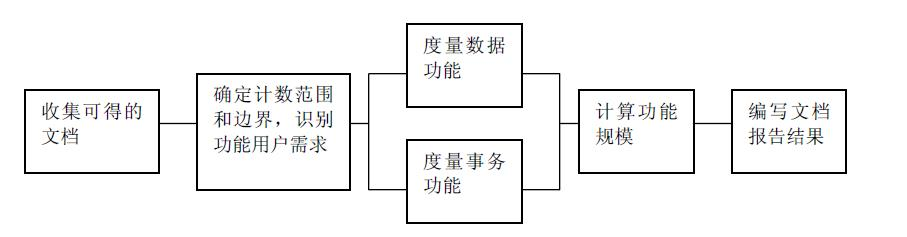
\includegraphics[width=10cm]{功能点计数过程.jpg}

\hypertarget{ux7b80ux5316ux529fux80fdux70b9ux4f30ux7b97ux6b65ux9aa4}{%
\subsubsection{简化功能点估算步骤:}\label{ux7b80ux5316ux529fux80fdux70b9ux4f30ux7b97ux6b65ux9aa4}}

\begin{enumerate}
\tightlist
\item
  确定功能点分析类型
\item
  识别分析范围和应用边界
\item
  计算数据类型功能点(Data Function)
\item
  计算交易类型功能点(Transaction Function)
\item
  计算功能点
\end{enumerate}

\hypertarget{ux4e09ux79cdsifpux8ba1ux7b97ux7c7bux578b}{%
\subsubsection{1:三种SiFP计算类型}\label{ux4e09ux79cdsifpux8ba1ux7b97ux7c7bux578b}}

\begin{itemize}
\tightlist
\item
  开发(Development )
\end{itemize}

\begin{description}
\item[]
\begin{description}
\tightlist
\item[]
DSFP = ADD + CFP
\end{description}
\end{description}

\begin{itemize}
\tightlist
\item
  应用 (Application or Baseline after the initial development)
\end{itemize}

\begin{description}
\item[]
\begin{description}
\tightlist
\item[]
ASFP = ADD
\end{description}
\end{description}

\begin{itemize}
\tightlist
\item
  更新/增强功能与维护 (Enhancement)
\end{itemize}

\begin{description}
\item[]
\begin{description}
\tightlist
\item[]
ESFP = ADD + CHG + DEL + CFP
\end{description}
\end{description}

%Screenshotfrom20221220202712.png

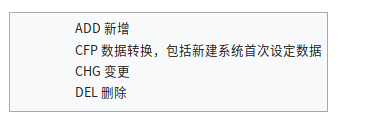
\includegraphics[width=10cm]{Screenshotfrom2022122020-31-37.png}

\hypertarget{ux8bc6ux522bux5206ux6790ux8303ux56f4ux548cux5e94ux7528ux8fb9ux754c}{%
\subsubsection{2:识别分析范围和应用边界}\label{ux8bc6ux522bux5206ux6790ux8303ux56f4ux548cux5e94ux7528ux8fb9ux754c}}

例子:用虚线标示系统边界:\\
%\href{文件:功能点计数P62_2.0.jpg}{500px}\\

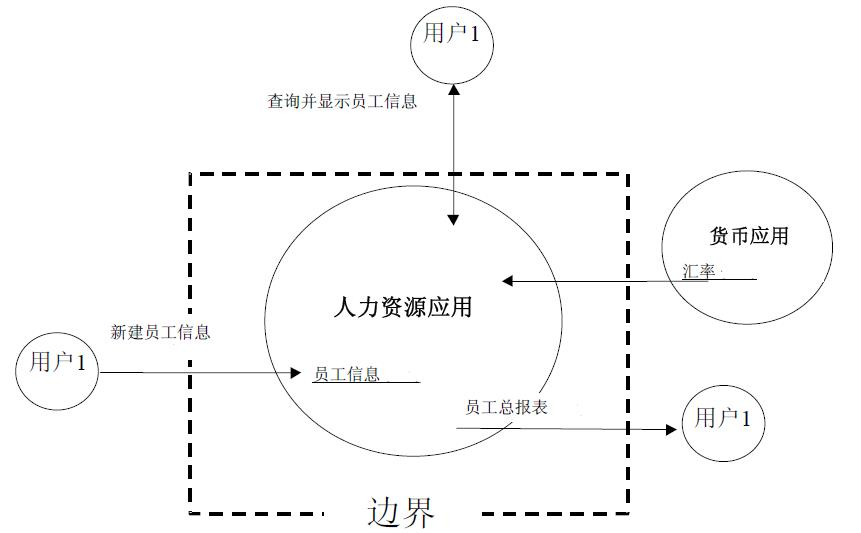
\includegraphics[width=10cm]{功能点计数P6220.jpg}

\hypertarget{ux8ba1ux7b97ux903bux8f91ux6587ux4ef6ux6570}{%
\subsubsection{3:计算逻辑文件数}\label{ux8ba1ux7b97ux903bux8f91ux6587ux4ef6ux6570}}

\begin{itemize}
\tightlist
\item
  关于计算规则,详见"逻辑文件"
\end{itemize}

\hypertarget{ux8ba1ux7b97ux57faux672cux8fc7ux7a0bux6570}{%
\subsubsection{4:计算基本过程数}\label{ux8ba1ux7b97ux57faux672cux8fc7ux7a0bux6570}}

\begin{itemize}
\tightlist
\item
  关于计算规则,详见"基本过程"
\end{itemize}

\hypertarget{ux8ba1ux7b97ux529fux80fdux70b9}{%
\subsubsection{5:计算功能点}\label{ux8ba1ux7b97ux529fux80fdux70b9}}

\begin{itemize}
\tightlist
\item
  每个逻辑文件 = 7.0 简化功能点
\item
  每个基本过程 = 4.6 简化功能点
\end{itemize}

\hypertarget{ux903bux8f91ux6587ux4ef6-logical-file}{%
\subsection{逻辑文件 Logical
File}\label{ux903bux8f91ux6587ux4ef6-logical-file}}

\textbf{(下面在计算实例里简称``实体'',方便理解)}

\begin{itemize}
\tightlist
\item
  用来储存内部或外部数据,是用户可识别的逻辑相关的数据组或控制信息组,在被度量应用边界内部维护。
\end{itemize}

\begin{description}
\tightlist
\item[]
(\textbf{用户可识别} -
用户可识别 -指数据或事务需求是被用户和软件开发人员双方共同认同并理解的。
例如:用户和软件开发人员双方都认同人力资源应用有维护和存储员工信息的功能。)
\end{description}

\hypertarget{ux6ce8ux610f}{%
\paragraph{注意}\label{ux6ce8ux610f}}

逻辑文件包括两类不同的用户需求数据:

\begin{enumerate}
\tightlist
\item
  功能性数据
\item
  非功能性数据
\end{enumerate}

功能性数据是用来满足用户功能需求的数据。例如,销售、银行账号、供应商、人员等信息。\\
非功能数据主要是为了满足易用性(支撑下拉菜单所需的数据,可输入数据的上下范围等);或性能方面(用于查询数据的索引index);或可维护性(配置参数)。\\
只有第一类功能性数据才算是逻辑文件。\\

\hypertarget{ux57faux672cux8fc7ux7a0b-elementary-process}{%
\subsection{基本过程 Elementary
Process}\label{ux57faux672cux8fc7ux7a0b-elementary-process}}

基本过程是对用户有意义的最小活动单元。例如:添加员工的用户需求包括建立工资和家属信息。只有添加所有员工信息,才能创建员工信息记录。单独添加一些信息使添加员工业务处于不持续状态,只有员工工资和家属信息都添加后,这个活动单元才能完成且业务处于稳定状态。

\hypertarget{ux8bc6ux522bux57faux672cux8fc7ux7a0b}{%
\subsubsection{识别基本过程}\label{ux8bc6ux522bux57faux672cux8fc7ux7a0b}}

为了识别基本过程,需要执行以下活动:

\begin{itemize}
\tightlist
\item
  把功能用户需求分解为最小活动单元,使其满足下面条件:

  \begin{itemize}
  \tightlist
  \item
    对用户有意义\\
    例如:功能用户需求要求在应用中添加新员工的能力。\\
  \item
    构成一个完整的事务\\
    例如:用户定义的员工信息包括工资和家属信息。如果家属人数大于零,添加员工信息时必须包括家属信息。本例中,添加员工信息(不包括添加地址、工资和家属信息)不满足本规则。\\
  \item
    自包含\\
    例如:除非输入所有的必需信息并且完成所有处理步骤,如验证、计算、更新ILFs,添加过程才是自包含的。\\
  \item
    让应用程序的业务保持持续状态\\
    例如:添加员工的用户需求包括建立工资和家属信息。只有添加所有员工信息,才能创建员工信息记录。单独添加一些信息使添加员工业务处于不持续状态,只有员工工资和家属信息都添加后,这个活动单元才能完成且业务处于持续状态。\\
  \end{itemize}
\end{itemize}

识别活动单元为基本过程需要满足以上所有规则。\\

\hypertarget{ux8bc6ux522bux57faux672cux8fc7ux7a0bux4e3bux8981ux76eeux7684}{%
\subsubsection{识别基本过程主要目的}\label{ux8bc6ux522bux57faux672cux8fc7ux7a0bux4e3bux8981ux76eeux7684}}

基本过程的主要目的可识别为下列情形的一种:

\begin{itemize}
\tightlist
\item
  改变应用行为
\item
  维护一个或多个ILFs
\item
  呈现信息给用户
\end{itemize}

\hypertarget{ux5b9eux4f8bux8bc6ux522bux57faux672cux8fc7ux7a0b-ep-elementary-process}{%
\subsection{实例:识别基本过程 (EP elementary
process)}\label{ux5b9eux4f8bux8bc6ux522bux57faux672cux8fc7ux7a0b-ep-elementary-process}}

下面是某预约网约车过程:

%Screenshotfrom20221220203338.png

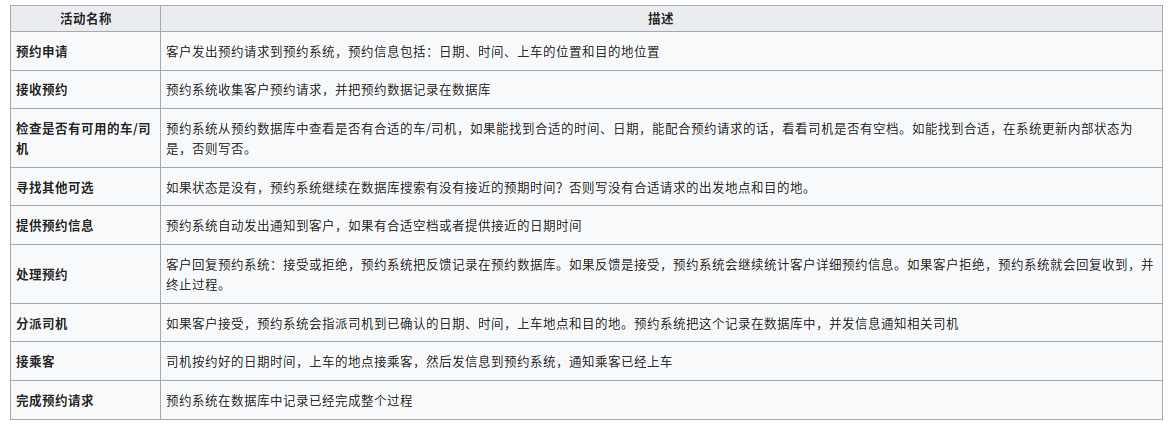
\includegraphics[width=10cm]{Screenshotfrom20221220203338.png}

\textbf{分析能否满足所有 EP 识别规则,判断能否独立成为基本过程 (EP
elementary process),部分例子}

\hypertarget{ux9884ux7ea6ux7533ux8bf7}{%
\subsubsection{预约申请}\label{ux9884ux7ea6ux7533ux8bf7}}

\begin{enumerate}
\tightlist
\item
  是否对用户有意义,客户功能需求的一部分?\textbf{是}
\item
  是否构成一个完整的事务?\textbf{否}:预约申请本身不是一个完整的交易,因为过程必须也包括预约请求信息,收到其它可选的档期这些步骤,都不可以分离。
\item
  是否自包含,可以独立存在?\textbf{否}:例如,接受预约申请;查看是否有档期,查看有没有其它接近的档期等,都是一些必须的相关步骤去完成这个基本过程。
\item
  是否让应用程序达到稳定状态?\textbf{否}:整个业务需求只能在收到预约信息,发送、接受、处理、反馈给客户才算是完成稳定状态。
\end{enumerate}

\hypertarget{ux5206ux6d3eux53f8ux673a}{%
\subsubsection{分派司机}\label{ux5206ux6d3eux53f8ux673a}}

\begin{enumerate}
\tightlist
\item
  是否对用户有意义,客户功能需求的一部分?\textbf{是}
\item
  是否构成一个完整的事务?\textbf{是}:分配到司机是一个完整的交易,包括收到司机的确认,把信息记录在系统中并通知司机。
\item
  是否自包含,可以独立存在?\textbf{是}:分配到司机本身可以独立存在。
\item
  是否让应用程序达到稳定状态?\textbf{是}:因为当司机被分配后,是完全满足业务的需要。
\end{enumerate}

\hypertarget{ux63a5ux4e58ux5ba2}{%
\subsubsection{接乘客}\label{ux63a5ux4e58ux5ba2}}

\begin{enumerate}
\tightlist
\item
  是否是客户功能需求?\textbf{是}
\item
  交易是否完整?\textbf{否}:接乘客本身不算一个完整的交易,因为预约系统必须也记录这个信息。
\item
  是否自包含,可以独立存在?\textbf{否}:确认预约申请是下面一个必须执行的过程,来完成这个基本过程。
\item
  是否让应用程序达到稳定状态?\textbf{否}:整个业务需求只能在和预约系统确认沟通,已经接到乘客,然后系统也把记录更新到预约系统才算完成。
\end{enumerate}

%Screenshotfrom2022122020-34-37.png

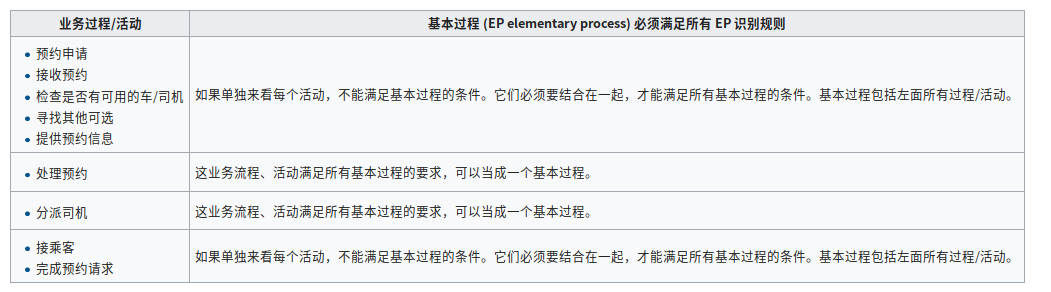
\includegraphics[width=10cm]{Screenshotfrom2022122020-34-37.png}


\hypertarget{ux4e0eux56fdux9645ux529fux80fdux70b9ifpugux7684ux504fux5dee}{%
\subsection{1.潜水学校:开发项目 }\label{ux4e0eux56fdux9645ux529fux80fdux70b9ifpugux7684ux504fux5dee}}

\hypertarget{ux63a5ux4e58ux5ba2}{%
\subsubsection{描述}\label{ux63a5ux4e58ux5ba2}}

一所潜水学校需要一套用来管理合同员工(教练)、设施、轮班工作的系统。目的:有效地管理教练在潜水设施和几艘旅游潜水船上有关潜水课程/短途潜水的轮班工作。 \\
\hypertarget{ux63a5ux4e58ux5ba2}{%
\subsubsection{功能需求}\label{ux63a5ux4e58ux5ba2}}

该系统将包括菜单界面和定期运行的批量处理等功能。\\
The system will consist of an online component based on a menu interface and a batch component that will run periodically. \\

\hypertarget{ux63a5ux4e58ux5ba2}{%
\subsubsection{RF01}\label{ux63a5ux4e58ux5ba2}}

为处理教练保险单文件,并符合法例,学校需要为每个合同员工储存以下资料: \\


\begin{itemize}
\tightlist
\item
  序列号(独特,作为索引, 不能重复)
\item
  姓名
\item
  居住地址
\item
  城镇
\item
  邮政编码
\item
  电话号码
\item
  是否持有航海执照
\end{itemize}

为了跟踪每个合同员工的“职业生涯”,学校决定给予他们以下分类: \\
1.“潜水长”
2.“助理教练”
3.“教练”

这些分类是固定的,并不会随着时间而转变:每个合同员工会按顺序分配到合适的类别,代表个人“职业生涯”的发展(例如,一个新员工开始是“潜水长”,随着时间的推移,他会成为“教练”)。\\

使用表单输入,显示,编辑和删除合同员工的数据。会有一个独立列表框,显示序列号、名和姓 (但没有附件明细),来选择要编辑、删除或详细查看的是哪位员工的数据。\\


用功能键激活所有的功能,并最终产生一个结果或错误信息。“删除合同员工”只是在逻辑上删除,没有数据会被物理删除,但会被标记为作废。只要有与其相关的工作班次,合同员工就不能被删除。 \\

\hypertarget{ux63a5ux4e58ux5ba2}{%
\subsubsection{RF02}\label{ux63a5ux4e58ux5ba2}}

%学校还需要管理设施(“潜水”、“船”或“橡皮艇-RD”),每一个设施都有独特的友好名称(例如:“潜水莫格利亚 diving-moneglia”、“潜水帕拉 diving_palau”、“蓝箭艇 blue-arrow-boat”、“格里大艇 goletta-boat”、“嘉莉花RD Genova_RD”等等)。\\

对于每种类型的设施,必须存储以下信息: \\

\begin{itemize}
\tightlist
\item
  设施识别名(独特,作为索引,不能重复)
\item
  描述
\item
  类型
\item
  它能容纳的人数
\item
  可用汽缸数
\item
  是否有厕所
\item
  是否有饮用水储备
\end{itemize}

必须创建表单来输入、显示、编辑和删除设施数据;如果有被分派到轮班,就不能删除设施。使用独立的列表(不显示附件细节),以便选择要编辑、删除或详细查看的数据,列表只展示:标识名称、描述、类型\\
用功能键来激活某功能,并最终生成错误或结果信息。 \\

\hypertarget{ux63a5ux4e58ux5ba2}{%
\subsubsection{RF03}\label{ux63a5ux4e58ux5ba2}}

最后,为了有效管理分派轮班(shift)的覆盖范围,学校需要处理合同员工以下轮班(shift)信息: \\

\begin{itemize}
\tightlist
\item
  工作轮班识别名(独特,作为索引,不能重复)
\item
  可用的合同员工编号(使用下拉框挑选)
\item
  提供本轮班可用的日期
\item
  可用期的开始日期
\item
  可用期的结束日期
\item
  首选设施(使用下拉框挑选)
\item
  状态(最初预设置为“预计轮班”)
\end{itemize}

必须创建表单来输入、显示、编辑和删除轮班(shift)的有效信息。为了方便选择对哪些数据进行编辑、删除或查看详细信息,会独立显示没有附件细节的数据列表(如,不显示可用性标识号,合同员工序列号)。用功能键将激活这功能,并最终生成错误/或结果信息。 \\

\hypertarget{ux63a5ux4e58ux5ba2}{%
\subsubsection{RF04}\label{ux63a5ux4e58ux5ba2}}

每个合同员工可以提供不止一个可用轮班(availability),每一个轮班最初都设定为“预计轮班tentative shift”状态。\\
当分配协调各合同员工的可用轮班作为一个“轮班(shift)”内的可用资源时,秘书处在一个“分配轮班 assigned shift”内使用特定命令选择(转换)所需的可用轮班(availability),她可以更改潜水期的开始和结束日期,并可以将之设定为“分派轮班”状态。删除“分派轮班”与删除“预计轮班”的功能/步骤类似。 \\


\hypertarget{ux63a5ux4e58ux5ba2}{%
\subsubsection{RF05}\label{ux63a5ux4e58ux5ba2}}

有以下查询:

1.找出合同员工中谁已经有许可证,因此能够以“船夫”的身份带队出海 - 显示属性:序列号。姓和名,和总人数。
2.选择当前某月份(或其他月份和年份)收到的所有可用合同员工——显示的属性:序列号、姓名、类别、可用期的开始日期和结束日期以及对设施的偏好。
3.根据档案中设施的数量和类型,(包括考虑潜水和船数量)计算学校管理的最大人数。
4.计算每个类别的员工人数(潜水主任;助理教练;教练):按类别列出总计和小计。
5.通过显示姓名和姓氏,显示最“忠诚”的员工,即年初以来提供最多可用时间段的前三名员工。
6.上面查询4的增强版: 通过类别细化——换句话说,不仅仅是显示数量,可选择某个类别的相关合同员工列表(姓和名)与其总数量。


\hypertarget{ux4f8bux5b50ux4e00-ux7b54ux6848ux4e0eux89e3ux8bfb}{%
\subsection{例子一:
答案与解读}\label{ux4f8bux5b50ux4e00-ux7b54ux6848ux4e0eux89e3ux8bfb}}

共三个实体:

\begin{enumerate}
\tightlist
\item
  合同员工
\item
  管理设施
\item
  轮班
\end{enumerate}

你可能会问:那些合同员工的职称是否也应该是一个实体?(因需要花工夫开发)\\
这不应该是一个实体,原因:人员的职称必须依赖人员的信息挂在一起,不可以独立存在,就好比我们要维护员工信息,假如也要维护员工的家属信息,这个家属信息就不能算另外一个实体,因为没有人员的话,家属是不能单独存在的。原则:不是根据是否要产生开发的工作量,而是从用户角度看,这个实体能否独立存在和维护。否则功能点的估算就只是根据个人对开发工作量的估计,而不是从用户角度看功能的客观判断。

每个实体对用户来讲,都有新增、展示、修改、删除4个功能。在人员管理里,还有一个功能是显示一个可选的列表,方便用户选择,这功能是增查改删以外的第五个功能。

设施管理也同样有这个列可选设备设施的一个展示框这第五个功能。

在轮班管理里面,除了增加、查看、修改、删除和展示外,它里面有两个下拉框功能:

\begin{enumerate}
\tightlist
\item
  让客户挑选相关设施的 Combo-box下拉框
\item
  让客户选人员的框
\end{enumerate}

你可能会问,这 2
个下拉框功能是否不应该算额外的功能,而是属于``轮班''的增删改查基本功能的一部分?\\
我们可以这样想:从用户的角度来看,如果没有这两个下拉框的功能,基本的增删改查功能是否可以实现;现在做了两个下拉框的功能,是额外的新增功能,更方便用户去选择,所以这两个算是额外两个功能。

也可参考IFPUG关于EI/EO/EQ 的识别要求;基本操作(elementary
process)必须符合以下三条之一:

\begin{enumerate}
\tightlist
\item
  使用独特处理逻辑,与应用中其他`行为'(EI/EO/EQ) 的处理逻辑不同
\item
  在该处理中识别出来的数据元素是与应用中其他`行为'(EI/EO/EQ)
  的数据元素不同
\item
  在该处理中引用的`实体'(ILF 和EIF) 与其他`行为'(EI/EO/EQ)
  所引用的不同
\end{enumerate}

它要列出所有合条件的数据元素进这下拉框,类似一个新的报表,所以算一个行为。基于同类原因,挑选相关设施的
Combo-box 下拉框,选择可用合同员工 Combo-box 下拉框, 等各自也算一个行为。

在轮班里,还有一个展示可选的轮班功能,另外是分配轮班功能。还有最后的
RF05 六个查询功能。

得出共 24(=5+5+6+2+6)行为,加 3实体, 所以按简化功能点每个实体 x7,每行为
x4.6 得出,共新增131.4(=3x7+24x4.6)简化功能点,详见下面列表:

%\href{文件:Ex1SoluScreenshot_2022-04-05_115926.jpg}{500px}

%Ex1SoluScreenshot_2022-04-05_115926.jpg

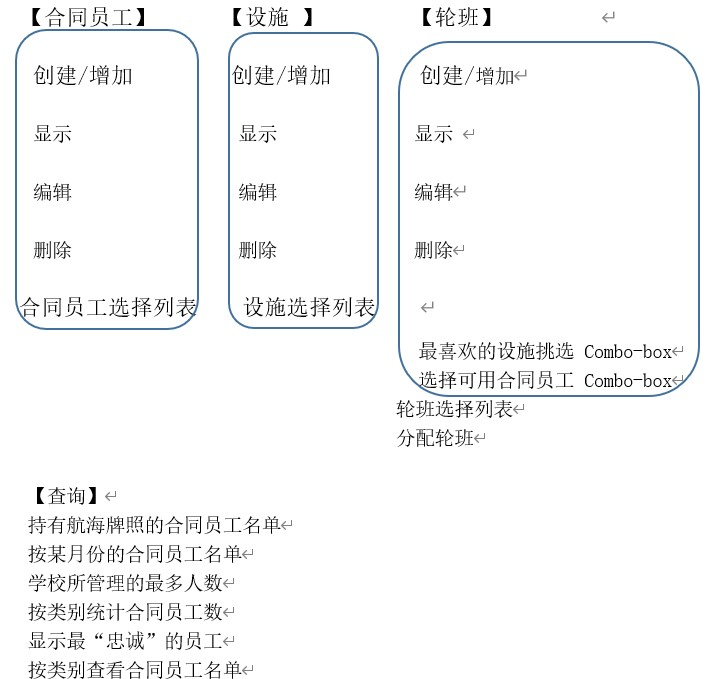
\includegraphics[width=10cm]{Ex1SoluScreenshot_2022-04-05_115926.jpg}

%\href{文件:微信截图_20220412130822.jpg}{550px}

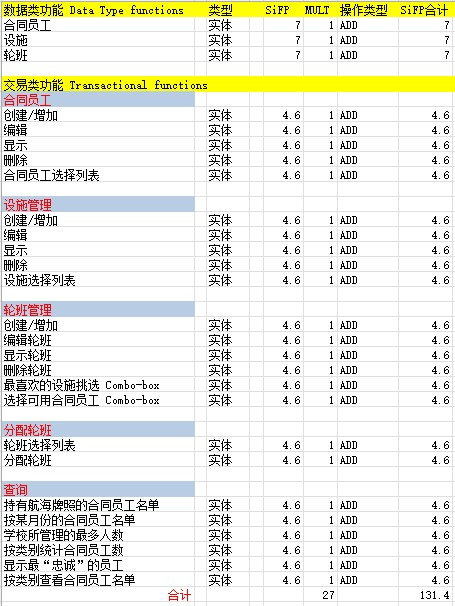
\includegraphics[width=10cm]{SifpEg1Screenshot_2023-03-15_204147.jpg}

\hypertarget{ux8ba1ux7b97ux529fux80fdux89c4ux6a21}{%
\subsubsection{计算功能规模}\label{ux8ba1ux7b97ux529fux80fdux89c4ux6a21}}

\begin{description}
\item[]
\begin{description}
\tightlist
\item[]
DSFP = ADD + CFP
\end{description}
\end{description}

因为没有数据转换,所以 CFP=0, 所以 DSFP = (110.4+21) +0 = 131.4 SiFP

因是首次开发, ASFP = ADD = 131.4 SiFP

\hypertarget{ux6f5cux6c34ux5b66ux6821femux9879ux76ee}{%
\subsection{2.潜水学校:FEM项目}\label{ux6f5cux6c34ux5b66ux6821femux9879ux76ee}}

\hypertarget{ux63cfux8ff0}{%
\subsubsection{描述}\label{ux63cfux8ff0}}

参照之前的潜水学校系统,对功能进行了增强,并提出了该软件的功能优化维护项目(FEM)。

\hypertarget{ux529fux80fdux9700ux6c42}{%
\subsubsection{功能需求}\label{ux529fux80fdux9700ux6c42}}

\hypertarget{rf01}{%
\paragraph{RF01}\label{rf01}}

用户想要取消合同员工删除功能。The user wants to eliminate the Contractor
delete function.

\hypertarget{rf02}{%
\paragraph{RF02}\label{rf02}}

在短途潜水里, 在潜水设施管理中能管理船上医生的存在或缺失。The
presence/absence of a ship doctor during excursions must be managed in
the file DIVING FACILITIES.

\hypertarget{rf03}{%
\paragraph{RF03}\label{rf03}}

出于税收和安全原因,不再需要删除可用轮班这项功能 For tax and safety
reasons the function to delete availability shifts will no longer be
required.

\hypertarget{rf04}{%
\paragraph{RF04}\label{rf04}}

用户还需要管理课程参与者信息和他们参加的那个短途潜水信息:\\
*管理参与者的信息包括:参与者ID,姓,名,出生日期,潜水执照,执照日期。\\
参加短途潜水:参与者ID。轮班编号,出游日,天数,最终考试是/否通过\\
*用列表框 (包括:参与者ID,姓,名)来选择轮班中的参与者。\\
*使用原本应用程序中已经有的列表框选择轮班。\\
*用功能键将激活这功能,并最终生成错误信息/结果。

用功能键初始填充课程参与者信息,参与者信息源自以前参与者信息的备份数据。

\hypertarget{rf05}{%
\paragraph{RF05}\label{rf05}}

用户还需要能够在课程结束时颁发出席证书给在短途潜水中登记的所有参与者。除了管理参与者基础数据外,还需要管理:参与者所登记的轮班、轮班日期、时长、教练的姓名和医生(如在场)的姓名。该功能使用原本应用程序中已经可用的功能:选择轮班。用功能键将激活这些功能,并最终生成错误/结果消息。

\hypertarget{rf06}{%
\paragraph{RF06}\label{rf06}}

用户还需要能够向合同员工颁发``教员身份参与证书'',其中的信息除了基础数据外还包括:轮班ID、教练ID、出游日、船医(如果有的话)。对于轮班选择,将使用原本应用程序中已经有的列表框。用功能键将激活这功能,并最终生成错误信息/结果。

\hypertarget{ux4f8bux5b50ux4e8c-ux7b54ux6848ux4e0eux89e3ux8bfb}{%
\subsection{例子二:
答案与解读}\label{ux4f8bux5b50ux4e8c-ux7b54ux6848ux4e0eux89e3ux8bfb}}

RF02 变动了潜水设施的内容,所以设施实体有变更。\\
因为设施的信息有变更,导致跟这实体相关的行为,包括新增、编辑、和展示这三行为都会有变更。

另外加了两个要管理的实体:

\begin{enumerate}
\tightlist
\item
  参与者
\item
  短途潜水
\end{enumerate}

不需要合同员工的删除功能,所以是个行为删除。

在参与者的管理,除了增加,改动,展示和删除四个功能以外,还有可以挑选参与者的下拉框功能。

两个证书的功能

\begin{enumerate}
\tightlist
\item
  给教练的证书
\item
  给参与者发证书
\end{enumerate}

对应每个短途潜水也需要有添加、改动、展示、删除的四功能。
那个删除轮班功能也被删掉了。

增加了两个实体 -\/-参与者 与 短途潜水旅行登记\\
Q: 为什么短途潜水旅行登记算一个实体?\\
A: 因它包括的信息都不能归入已有的 【参与者】 【合同员工】 【设施
】【轮班】实体里,例如那位参与者参加了那个班,考试分数等。
也可参考IFPUG关于ILF/EIF (实体)的识别要求;必须符合以下条件:

\begin{enumerate}
\tightlist
\item
  数据的集合必须是逻辑相关的并且是用户可以识别
\item
  这些数据或者控制信息必须是在本应用的边界内被维护
\end{enumerate}

总结:

\begin{itemize}
\tightlist
\item
  实体方面增加了2 实体; 设施实体有变更。
\item
  行为方面主要的在短途潜水旅行方面增加了4 增删改查的功能和。5
  参与者的功能(因为在里面加了一个下拉框功能),增加了2
  证书功能。改动了设施的增加、编辑、和展示,三个行为,删掉了两个行为。
\end{itemize}

所以动态功能点是增加的功能点64.6 (=2x7 +(4+2+5)x4.6),变更 20.8
(=3x4.6),删除9.2 (=2x4.6),总共的动态简化功能点 94.6。

静态功能点依据上面练习一那的131.4,加上增加的功能点 64.6,减掉
删除功能点 9.2,得出变更后静态功能点 186.8。

%\href{文件:Ex2XlsScreenshot_2022-04-05_143941.jpg}{550px}

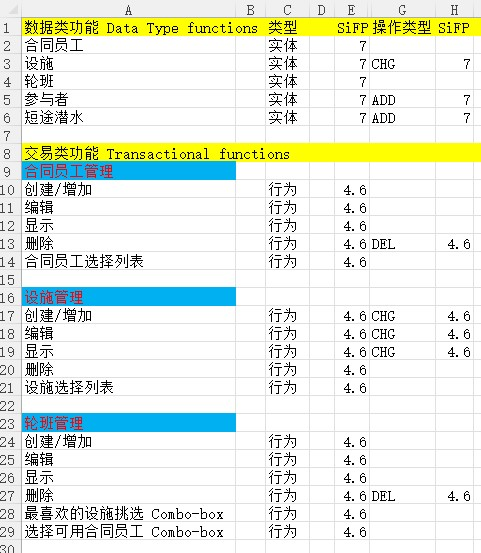
\includegraphics[width=10cm]{Ex2XlsScreenshot_2022-04-05_143941.jpg}

%\href{文件:Ex2XlsPt2of2Screenshot_2022-04-05_143941.jpg}{550px}

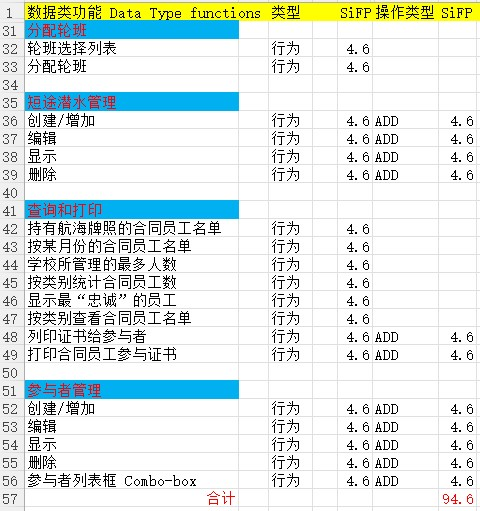
\includegraphics[width=10cm]{Ex2XlsPt2of2Screenshot_2022-04-05_143941.jpg}

\hypertarget{ux8ba1ux7b97ux529fux80fdux89c4ux6a21-1}{%
\subsubsection{计算功能规模}\label{ux8ba1ux7b97ux529fux80fdux89c4ux6a21-1}}

\begin{description}
\item[]
\begin{description}
\tightlist
\item[]
ESFP = ADD + CHG + DEL + CFP
\end{description}
\end{description}

因为有数据转换:初始填充课程参与者信息作为一个基本过程,所以 CFP=4.6

\begin{description}
\tightlist
\item[]
ESFP = (64.6 + 20.8 + 9.2) + 4.6 = 94.6 + 4.6 = 99.2 SiFP
\end{description}

软件开发后的静态功能点: ASFPA = ASFPB + ADD - DEL = 131.4 + 64.6 - 9.2
= 186.8 SiFP


\hypertarget{ux4e0eux56fdux9645ux529fux80fdux70b9ifpugux7684ux504fux5dee}{%
\subsection{与国际功能点(IFPUG)的偏差}\label{ux4e0eux56fdux9645ux529fux80fdux70b9ifpugux7684ux504fux5dee}}

例子:

\begin{itemize}
\tightlist
\item
  新开发某会计付款系统
\item
  实体: 包括管理 发票 ,付款,供货商。
\item
  行为:包括对每个实体的展示,增加,修改,和删除/取消
\item
  使用IFPUG 数 EI, EO, EQ, ILF, EIF
  每类的调整前功能点数,加起来得出调整前功能点数FP=82
  (如想多了解IFPUG如何计算复杂度,参考附件)
\item
  使用SiFP 估算实体和行为数,计算得出 FP=104
\end{itemize}

%\href{文件:FPA_S11.jpg}{500px}

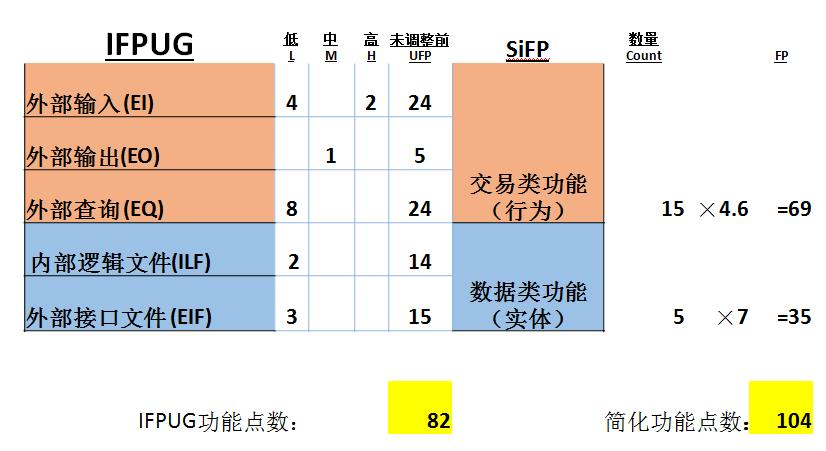
\includegraphics[width=10cm]{FPAS11.jpg}

\begin{itemize}
\tightlist
\item
  IFPUG / SiFP
  得出的实体数量,与行为数量都一样 (实体(=ILF+EIF)=5  行为
  (=EI+EO+EQ)=15)
\item
  因为简化功能点只是不区分实体与行为的复杂度(高中低),取平均值,原理一样,虽然个别估算有差异,但平均下来与IFPUG的估算没有结构性偏差
\end{itemize}

